\documentclass[12pt,a4paper]{article}

\usepackage[utf8]{inputenc}
\usepackage[T1]{fontenc}
\usepackage[francais]{babel}
\usepackage{setspace}
\usepackage{graphicx}

\title{Cahier des besoins - Mesure du rythme cardiaque à partir du flux vidéo de la Kinect 2}

\author{Hereiti \bsc{Hatitio} - Anta \bsc{Mbaye} - Maxime \bsc{Vincent} - Jean-Baptiste \bsc{Rey}}

\begin{document}
\maketitle

\tableofcontents
\newpage

\section*{Introduction}

Ce projet a pour objectif d'acquérir l'activité cardiaque d'une personne sans contact, uniquement par le biais d'un flux vidéo provenant d'une caméra.
Il sera possible de suivre une ou plusieurs personnes, éventuellement en mouvement, en reconnaissant préalablement leur visage. Un algorithme calculant les pulsations sera appliqué sur les zones suivies, et permettra d'obtenir une estimation du rythme cardiaque du ou des sujets filmés. Les résultats seront stockés sur la machine exécutant le programme et éventuellement envoyés vers des appareils distants.  

\section{Besoins fonctionnels}
Pour spécifier les fonctionnalités proposées et les services à rendre par notre projet, nous avons défini trois grands besoins fonctionnels : récupérer un flux vidéo, l'analyser pour interpréter le rythme cardiaque et sortir le résultat.

\subsection{Récupérer un flux vidéo}
Notre client nous a proposé d'utiliser Kinect 2 pour notre projet : elle présente les avantages de posséder des algorithmes de tracking dans son API et un flux infrarouge, en plus des flux classiques RGB.

Un problème s'est vite présenté : l'API de Kinect 2 est utilisable uniquement sur Windows 8. Nous avons donc eu deux alternatives : changer de périphérique d'entrée et utiliser une webcam, ou utiliser libfreenect2 sur Linux et implémenter nous-même des algorithmes de tracking avec opencv 2.4.

La kinect 2 nous servirait de caméra HD (1080p) en utilisant le flux infrarouge. Ce dernier nous permettra de confronter les résultats du RGB. Nous n'avons pas pu encore tester un flux infrarouge.

\subsection{Analyser un flux vidéo pour interpréter le rythme cardiaque}
Ce besoin fonctionnel principal est divisé en différents sous-besoins fonctionnels.

\subsubsection{Traiter le flux vidéo généré par une caméra}

Appliquer l'algorithme de tracking sur le flux vidéo d'une webcam (RGB ou infrarouge) ou de kinect 2.

\subsubsection{Détecter la zone de traitement}

Reconnaître au moins un visage, ou plus, l'algorithme de tracking de la kinect 2 sur Windows 8 étant par exemple capable de prendre en compte six personnes.
L'analyse du rythme cardiaque semble plus efficace (voir prototype) si nous isolons une zone du front.
Si nous rencontrons une difficulté pour le suivi des visages, une alternative serait de tracer un cadre pour que la personne place son visage dans cette zone à analyser.

\subsubsection{Suivre la zone de traitement}

Suivre la zone de traitement lorsque la ou les personnes sont en mouvement. Il est possible de rencontrer une difficulté dans le cas ou plusieurs personnes se chevauchent en se déplaçant, il est possible alors de déterminer une zone de mouvement pour chaque personne. Celle ci limite la zone ou le calcul s'effectuera. Si un sujet quitte sa zone attribuée alors le calcul s'arrête jusqu'à ce que la personne revienne dans son cadre.  Cette zone dépendra de l'angle de vision de la caméra.\\

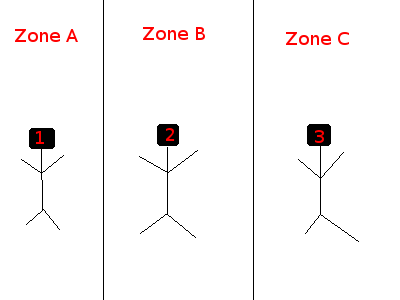
\includegraphics[scale=0.60]{zone_mouvement.png}

\textit{Image tirée d'une publicité Japonaise
}
\subsubsection{Identifier la ou les personnes}

Donner un identifiant numérique à chaque personne détectée : utile pour l'affichage des résultats dans le cas où le programme récupère plusieurs rythmes cardiaques.


\subsection{Affichage du résultat}

Trois cas sont envisageables : Le premier consiste à afficher sur une console et écrire dans un fichier log l'entier représentant la pulsation.
Le deuxième consiste à calculer et afficher le nombre de battements par minute dans les mêmes conditions que précédemment. Le troisième consiste à afficher sur une nouvelle fenêtre (GUI) une courbe de pulsation avec possibilité d'envoyer les résultats sur le réseau.\newline

 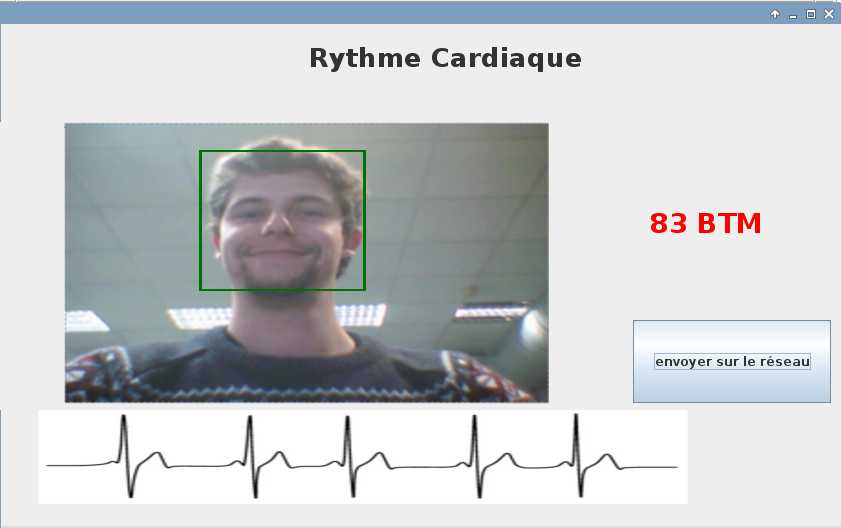
\includegraphics[scale=0.5]{gui.png}
\textit{Interface graphique possible.}
\newpage
Le rythme cardiaque obtenu pourra être utilisé sur d'autres appareils externes au programme. 
Nous enverrons donc un entier non chiffré en utilisant le protocole OSC ou LSL qui sera encapsulé dans une trame TCP. Les protocoles OSC et LSL permettent la synchronisation et facilitent le traitement coté client.

On pourra implémenter une architecture de Client-Serveur. L'ordinateur effectuant l'analyse sera considéré comme le serveur et les autres appareils comme les clients.

\subsubsection{Afficher des messages d'erreurs}

Possibilité d'afficher des messages d'avertissement pour l'utilisateur dans le cas où :

\begin{enumerate}
\item [] - Chevauchement de personnes
\item [] - Aucun utilisateur devant la caméra
\item [] - Perte du tracking
\item [] - Aucune caméra détectée 
\item [] - Impossibilité d'envoyer les données (protocole TCP)
\item [] - Front indétectable

\end{enumerate}
\newpage
\subsection{Schéma UML}
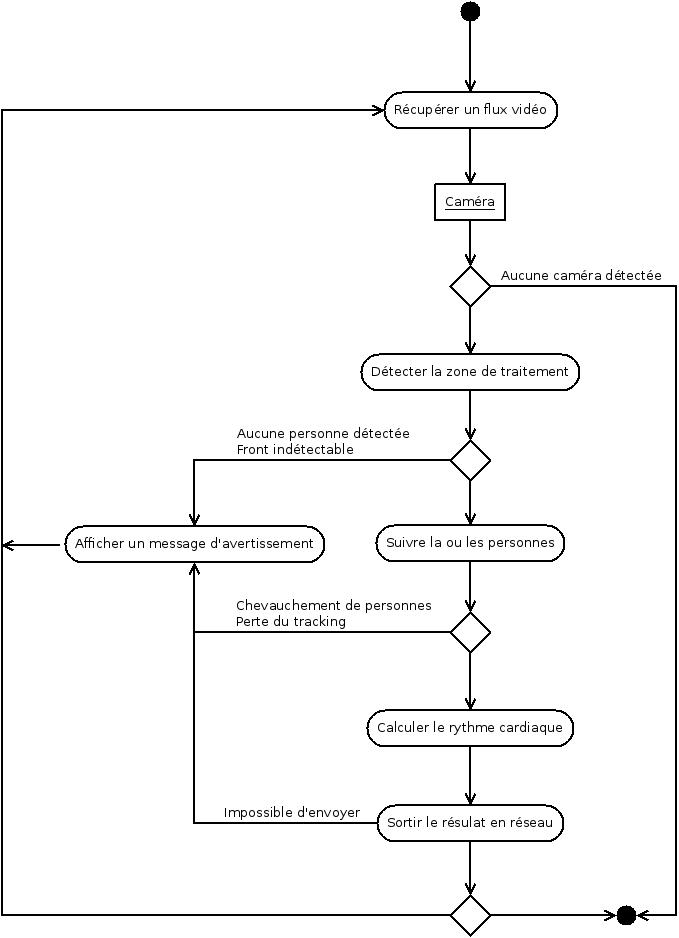
\includegraphics[scale=0.5]{uml.jpeg}
\newpage

\section{Besoins non fonctionnels}

Les besoins non fonctionnels de notre projet se résument en trois parties également.
\subsection{Portabilité}
Le programme doit être portable et modulaire. Notre programme sera découpé en plusieurs parties indépendantes les unes des autres. Ceci assurera la maintenabilité. Par exemple si un algorithme de tracking plus performant venait à être créé il pourrait remplacer le notre.

\subsection{Performance}

\subsubsection{Précision du rythme cardiaque}

En testant différents algorithmes de calcul de rythme cardiaque nous prendrons une marge d'erreur de cinq battements par minute. Pour vérifier nos valeurs, nous utiliserons un capteur arduino ou une électrocardiographie pour avoir de meilleur résultats.
\subsubsection{Temps du traitement}

Différents tests ont montré qu'il fallait un temps de calcul initial pour pouvoir obtenir les pulsations. Le calcul s'effectue au même moment que la scène filmée, l'affichage quant à lui se fait en différé. Ce temps varie entre 15 et 30 secondes.

\subsection{Ethique}

Notre programme a pour but de calculer le rythme cardiaque d'une personne filmée. Il est donc possible que cette personne n'accepte pas d'être filmée ou que son rythme cardiaque soit visible. De ce fait, un message au lancement du programme apparaîtra prévenant l'utilisateur.
\newpage
\subsection{Logiciel et système d'exploitation}

\subsubsection{OpenCV}

Nous utiliserons la version 2.4 d'OpenCV qui est portable sur Linux, Windows et Mac.

\subsubsection{libfreenect2}

La bibliothèque libfreenect2 est une alternative libre aux pilotes microsoft permettant l'accès aux flux RG et infrarouge de la kinect 2, elle nécessaire en cas d'utilisation de cette caméra.


\subsubsection{Système d'exploitation}

Notre programme sera compatible avec les distributions : 
\begin{enumerate}
\item[] - Linux Ubuntu 14.04
\item[] - Windows 7, 8 et 8.1
\end{enumerate}
Pour Windows si la kinect 2 est utilisée, Windows 8 ou 8.1 sera obligatoire.

\subsection{Test}
Les différents tests disponibles dans le dépôt nécessitent l'installation d'OpenCV.
Les tests ont été effectués avec une caméra Creative WebCam Live!(640x480 pixels), une caméra logitech QuickCam Chat (352 x 288 pixels) ainsi qu'avec les webcams intégrées de nos Ordinateurs portables respectif. (HP pavillon dv6, DELL inspiron 15R[1280x720 pixels])

Nous n'avons pas pu tester la kinect 2 car nous avons rencontré des difficultés pour l'utiliser. En effet la kinect 2 a besoin de plusieurs paramètres pour être exécutée.
Il faut installer la libfreenect2, posséder un port USB 3 et avoir une carte graphique avec le bon pilote pour pouvoir s'en servir en tant que Webcam.
Il faut une carte graphique NVIDIA ou ATI. La technologie optimus de NVIDIA est mal gérée par toute les distributions de linux. 

Voici une liste d'algorithmes que nous avons testé afin de faire une étude de faisabilité : 

\begin{enumerate}

\item[] - FaceTracker en C++ 
créé par Jason Saragih \\(http://jsaragih.org/) et maintenu par Kyle McDonald\\ (http://kylemcdonald.net/)

Le tracking de ce programme permet de suivre une personne. Il est fluide (10 frames secondes) avec la caméra Créative
\newline
\item[] - HearMonitor en Python par Mossblaser \\(https://github.com/mossblaser/HeartMonitor).


Ce programme calcule le rythme cardiaque d'une personne immobile. En appuyant sur la touche espace, la zone de traitement est mise à jour dans le cas où la personne s'est déplacée. Le calcul du rythme cardiaque se fait sur une fenêtre de trente secondes. 
Une fois opérationnel, la précision contient un écart de l'ordre de dix battements minutes.

\item[] - MultiTrackingPhoto en python auteur Inconnu 

Le programme prend en paramètre une photo et détecte les visages sur celle ci.
Son exécution est de l'ordre de 0.3 seconde pour détecter une vingtaine de visages.
\newline
 \item[] - Webcam-pulse-detector écrit par NASA Glenn Research Center \\(http://www.nasa.gov/centers/glenn)

Ce programme calcule avec une précision de cinq battements par minutes d'écart après trente secondes d'initialisation.

\end{enumerate}

Les différents tests que nous avons effectué nous ont montré qu'une caméra possédant une résolution de 352 x 288 pixels donnent des résultats plus précis qu'une webcam de résolution de 1280 x 720 pixels. 
\subsection{Diagramme de Gantt}
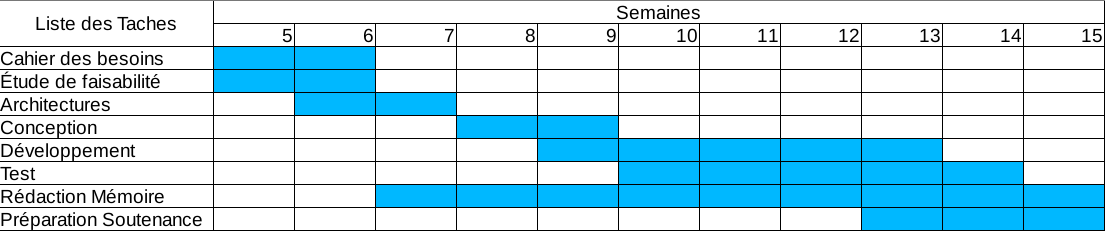
\includegraphics[scale=0.40]{Gantt.png}
La distribution des tâches n'a pas encore été décidé avec précision.\\ Elle sera effectuée au cours de la phase de conception.


\end{document}
